\chapter{Interactions}

Les diagrammes de séquences suivants ne reflètent que l'idée générale des algorithmes employés dans l'implémentation par défaut... Le scénario suivant montre un client qui accède à un objet distant via un registre connecté à un serveur de nom.

\section{Côté client}
\begin{figure}[H]
\begin{center}
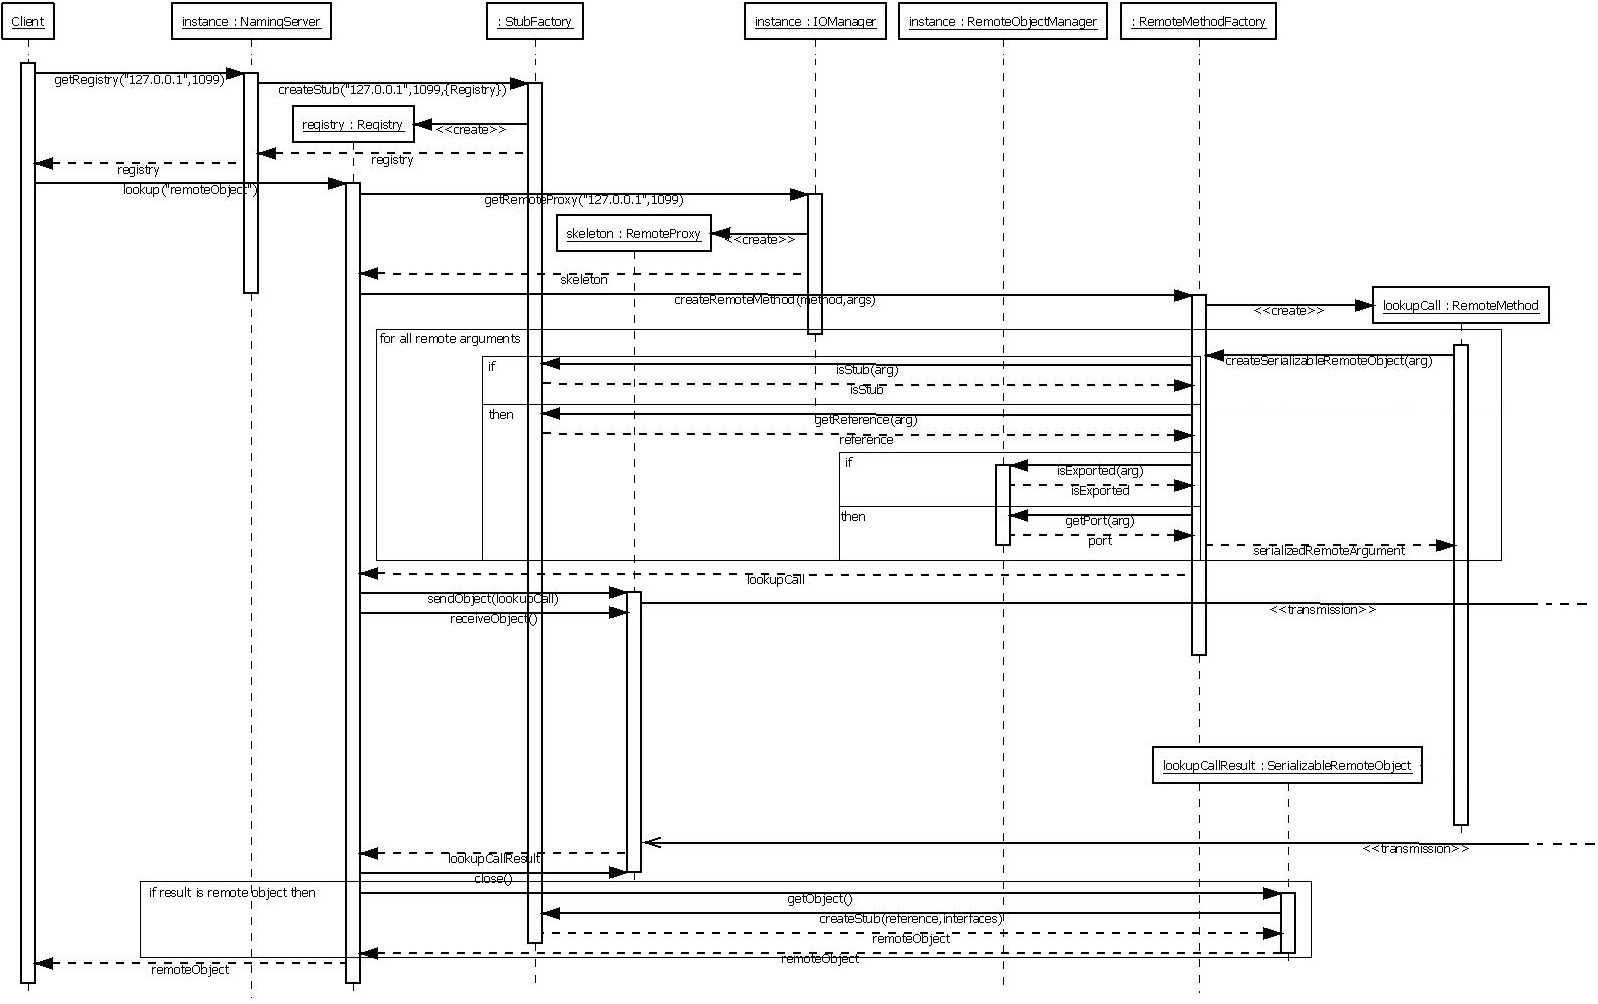
\includegraphics[scale=0.4,angle=90]{img/diag_sequence_client.jpeg}
\caption{Diagramme de séquence}
\end{center}
\end{figure}
\medskip
Le client récupère d'abord un stub connecté au registre (serveur de nom) distant, puis récupère un objet du serveur.

\section{Côté serveur}
Ici la méthode de createSerializableRemoteObject est simplifié afin de rendre le diagramme plus lisible (cf. client).
\begin{figure}[H]
\begin{center}
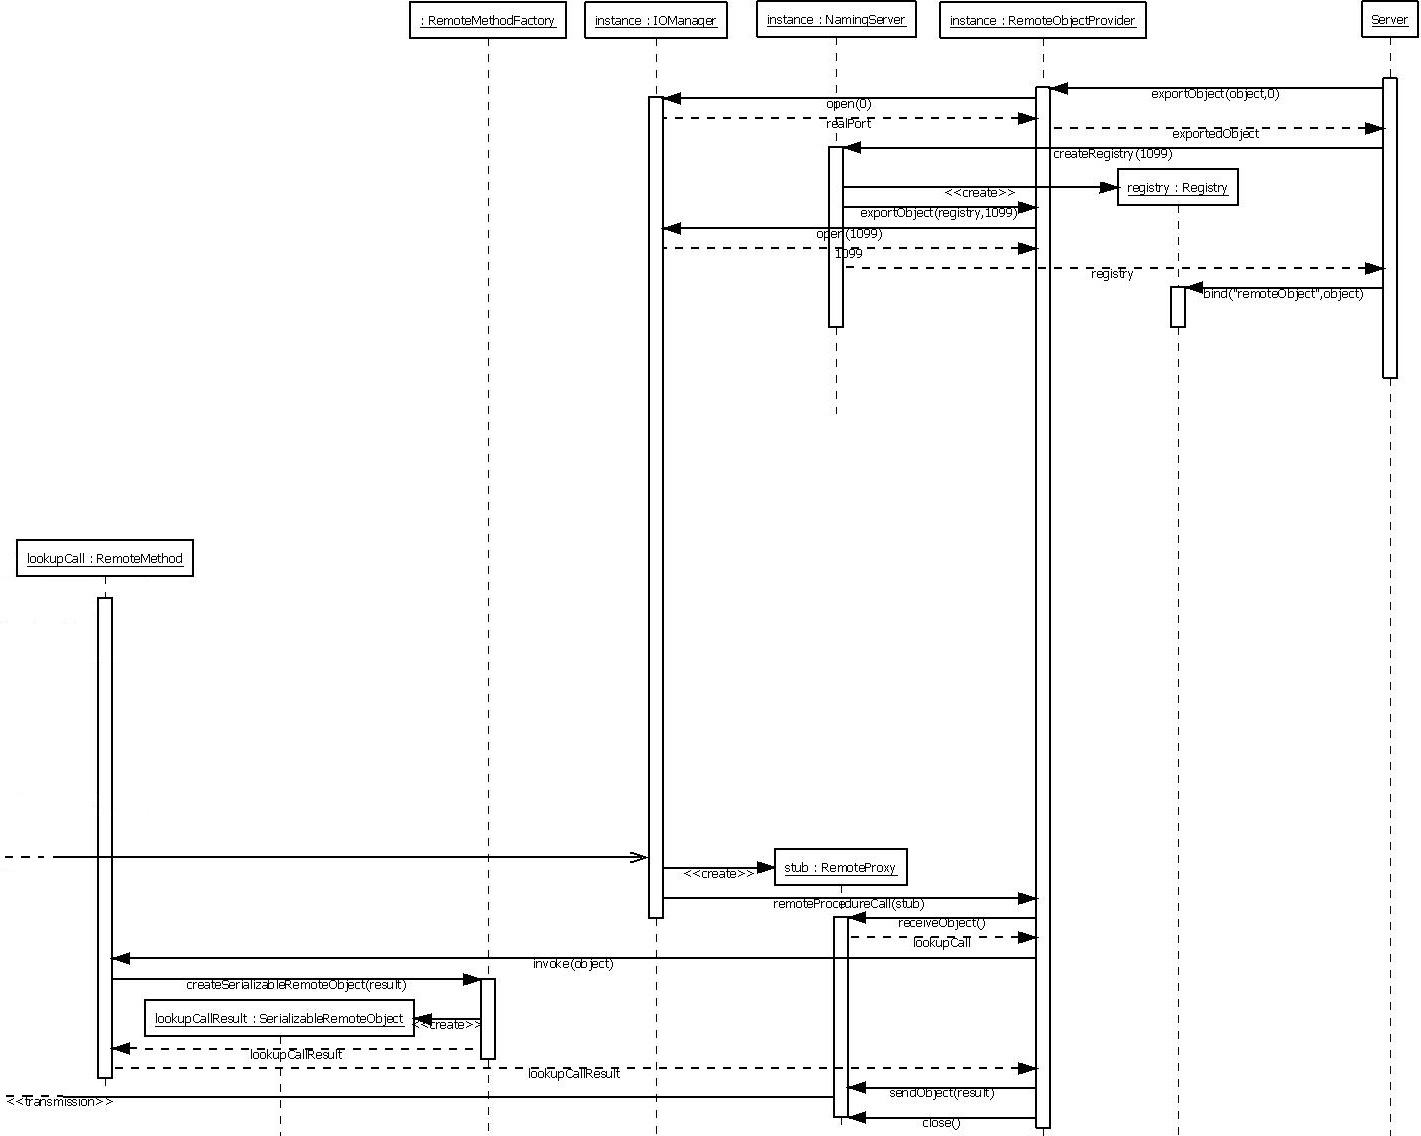
\includegraphics[scale=0.5,angle=90]{img/diag_sequence_server.jpeg}
\caption{Diagramme de séquence}
\end{center}
\end{figure}

